
\chapter[Bài tập: Quá trình biến đổi lực của con lắc lò xo chịu tác dụng lực cản]{Bài tập: Quá trình biến đổi lực của con lắc lò xo chịu tác dụng lực cản}
\section{Lý thuyết}
\subsection{Lực đàn hồi}
Độ lớn của lực đàn hồi bằng tích của độ cứng và độ biến dạng của lò xo so với chiều dài tự nhiên.
\begin{equation*} 
	F_\text{đh}=k\left| \Delta l\right|=k\left| l-l_0\right|, 
\end{equation*}
trong đó:
\begin{itemize}
	\item  $k$ là độ cứng của lò xo,
	\item  $\Delta l$ là độ biến dạng của lò xo,
	\item $l$ là chiều dài của lò xo sau khi bị biến dạng,
	\item $l_0$ là chiều dài tự nhiên của lò xo.
\end{itemize}
\subsection{Lực hồi phục}
Độ lớn của lực hồi phục bằng tích của độ cứng và li độ của vật.
\begin{equation*} 
	F_\text{hp}=k\left|  x \right|, 
\end{equation*}
trong đó:
\begin{itemize}
	\item  $k$ là độ cứng của lò xo,
	\item  $x$ là li độ của vật.
	
\end{itemize}
\subsection{Năng lượng con lắc lò xo}
\begin{equation*} 
	W=\dfrac{1}{2}kA^2, 
\end{equation*}
trong đó:
\begin{itemize}
	\item  $k$ là độ cứng của lò xo,
	\item  $A$ là biên độ,
	\item $W$ là năng lượng con lắc lò xo.
\end{itemize}

\subsection{Đặc điểm của con lắc lò xo chịu tác dụng của lực cản}
\begin{itemize}
	\item  Khi chịu tác dụng của lực cản, dao động có biên độ giảm dần theo thời gian.
	\item Nguyên nhân: Do khi dao động của vật chịu tác dụng của lực cản, lực cản sẽ làm cho cơ năng của vật giảm dần theo thời gian nên biên độ cũng giảm dần theo thời gian.
	\item Nếu \textbf{lực cản nhỏ} thì chu kỳ dao động của vật vẫn bằng chu kỳ dao động khi không có lực cản.	
\end{itemize}



\section{Mục tiêu bài học - Ví dụ minh họa}
\begin{dang}{Mô tả được quá trình dao động\\ của con lắc lò xo\\ khi chịu tác dụng của lực cản. 
	}
	
	
	\viduii{2}{Con lắc lò xo chịu tác dụng của lực cản thì các đại lượng nào sau đây giảm liên tục theo thời gian?
		
		\begin{mcq}(2)
			\item Biên độ và tốc độ.
			\item Biên độ và gia tốc.
			\item Li độ và tốc độ.
			\item Biên độ và cơ năng
		\end{mcq}
	}
	{\begin{center}
			\textbf{Hướng dẫn giải}
		\end{center}
		
		Con lắc lò xo chịu tác dụng của lực cản thì biên độ và cơ năng giảm liên tục theo thời gian.
		
		\textbf{Đáp án: D.}
	}
	\viduii{2}{ Đặc điểm của dao động con lắc lò xo khi chịu tác dụng của lực cản là 		
		\begin{mcq}
			\item khi ở vị trí cân bằng, động năng luôn không đổi.
			\item biên độ là hằng số.
			\item cơ năng giảm dần theo thời gian.
			\item cơ năng không thay đổi theo thời gian.
		\end{mcq}
	}
	{\begin{center}
			\textbf{Hướng dẫn giải}
		\end{center}
		
		
		Đặc điểm của dao động con lắc lò xo khi chịu tác dụng của lực cản là cơ năng giảm dần theo thời gian.
		
		\textbf{Đáp án: C.}
	}
\end{dang}
\begin{dang}{Xác định vị trí cân bằng mới,\\ vận tốc cực đại của con lắc lò xo\\ chịu tác dụng của lực cản}
	\ppgiai{
		\begin{center}
			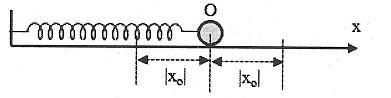
\includegraphics[scale=0.8]{../figs/VN12-PH-03-A-002-4-V2-1.jpg}
		\end{center}
		1. Vị trí cân bằng mới
		
		Con lắc lò xo chuyển động trên phương nằm ngang. Khi có lực ma sát tác động vào vật sẽ làm cho vị trí cân bằng của vật dịch chuyển.
		
		Gọi $x_0$ là vị trí cân bằng mới. Tại vị trí cân bằng mới thì $\vec{F}_{\text{đh}}+\vec{F}_{\text{ms}}=0$ hay $\vec{F}_{\text{đh}}=-\vec{F}_{\text{ms}}$.
		
		Về độ lớn: $F_{\text{đh}}=F_{\text{ms}}$ hay $k\left| x_0\right| =\mu mg\Rightarrow  \left| x_0\right|=\dfrac{\mu mg}{k}$.
		
		Vị trí cân bằng mới cách vị trí cân bằng cũ một đoạn là
		\begin{equation*} 
			\left| x_0\right|=\dfrac{\mu mg}{k}.
		\end{equation*}
		
		2. Vận tốc cực đại
		
		Vận tốc của vật ở vị trí cân bằng mới cũng chính là vận tốc cực đại:
		
		$\dfrac{1}{2}kA^2=\dfrac{1}{2}kx_0^2+\dfrac{1}{2}mv_\text{max}^2+\mu mg(A-x_0)$ với $x_0=\dfrac{\mu mg}{k}$.
		
		Suy ra:
		\begin{equation*} 
			v_\text{max}=\sqrt{\dfrac{k}{m}}\left(A-x_0\right)=\omega \left(A-x_0\right).
		\end{equation*}
		
	}	
	\viduii{2}{ Một con lắc lò xo gồm vật nhỏ khối lượng $\text{500}\ \text{g}$ và lò xo có độ cứng $k=100\ \text{N/m}$. Vật nhỏ được đặt trên giá đỡ cố định nằm ngang dọc theo trục lò xo. Hệ số ma sát trượt giữa giá đỡ và vật nhỏ là $\text{0,2}$. Lấy $g=10\ \text{m/s}^2$. Vị trí cân bằng mới cách vị trí cân bằng cũ một khoảng là 
		
		\begin{mcq}(4)
			\item $2\ \text{cm}$.
			\item $1\ \text{cm}$.
			\item $4\ \text{cm}$.
			\item $3\ \text{cm}$.
		\end{mcq}
	}
	{\begin{center}
			\textbf{Hướng dẫn giải}
		\end{center}
		
		$x_0=\dfrac{\mu mg}{k}=\text{0,01}\ \text{m}=1\ \text{cm}$.
		
		\textbf{Đáp án: B.}
	}
	\viduii{3}{Một con lắc lò xo gồm vật nhỏ khối lượng $\text{0,02}\ \text{kg}$ và lò xo có độ cứng $k=1\ \text{N/m}$. Vật nhỏ được đặt trên giá đỡ cố định nằm ngang dọc theo trục lò xo. Hệ số ma sát trượt giữa giá đỡ và vật nhỏ là $\text{0,1}$. Ban đầu giữ vật ở vị trí lò xo bị nén 10 cm rồi buông nhẹ để con lắc dao động tắt dần. Lấy $g=10\ \text{m/s}^2$. Tốc độ lớn nhất vật đạt được trong quá trình dao động là 
		\begin{mcq}(4)
			\item  $40\ \text{cm/s}$.
			\item  $40\sqrt{2}\ \text{cm/s}$.
			\item  $20\ \text{cm/s}$.
			\item  $20\sqrt{2}\ \text{cm/s}$.
		\end{mcq}
	}
	{\begin{center}
			\textbf{Hướng dẫn giải}
		\end{center}
		
		Tốc độ lớn nhất vật nhỏ đạt được trong quá trình dao động khi vật ở vị trí lực đàn hồi cân bằng với lực ma sát, tức là khi đó vật ở vị trí cân bằng mới.
		
		Định luật bảo toàn năng lượng trong quá trình dao động:
		
		$\dfrac{1}{2}kA^2=\dfrac{1}{2}kx_0^2+\dfrac{1}{2}mv_\text{max}^2+\mu mg(A-x_0)$ 
		
		Với $x_0=\dfrac{\mu mg}{k}=\text{0,02}\ \text{m}$.
		
		$\Rightarrow v_\text{max}=\sqrt{\dfrac{k}{m}}\left(A-x_0\right)=\omega \left(A-x_0\right)=40\sqrt{2}\ \text{cm/s}$.
		
		\textbf{Đáp án: B.}
	}
	
	
\end{dang}

\begin{dang}{Xác định  độ giảm biên độ\\ của con lắc lò xo sau mỗi chu kì, tổng số dao động thực hiện, tổng quãng đường\\ và tổng thời gian từ lúc bắt đầu dao động cho đến khi dừng hẳn}
	\ppgiai{
		1. Độ giảm biên độ
		
		Ta chỉ xét dao động tắt dần chậm nên độ giảm biên độ sau một chu kì rất nhỏ:
		
		$\Delta A=A-A'\Rightarrow A+A'=2A$, với $A$ là biên độ lúc đầu, $A'$ là biên độ lúc sau.
		
		Độ giảm cơ năng sau một chu kì bằng công thức của lực ma sát thực hiện trong chu kì đó:
		
		$W=\dfrac{1}{2}kA^2-\dfrac{1}{2}kA'^2=F_\text{ms}4A\Rightarrow \Delta A=\dfrac{4F_\text{ms}}{k}=\dfrac{4\mu mg}{k}$.
		
		\begin{itemize}
			\item Độ giảm biên độ sau mỗi chu kì: 
			\begin{equation*} \Delta A=\dfrac{4F_\text{ms}}{k}=\dfrac{4\mu mg}{k}.  	\end{equation*}
			
			\item Độ giảm biên độ sau nửa chu kì:  
			
			\begin{equation*}	\dfrac{\Delta A}{2}=\dfrac{2F_\text{ms}}{k}=\dfrac{2\mu mg}{k}.\end{equation*}
			\item Biên độ dao động còn lại sau n chu kì: 
			
			\begin{equation*} A_\text{n}=A-n\Delta A.\end{equation*}
		\end{itemize}
		
		2. Tổng số dao động thực hiện được
		\begin{equation*}
			N=\dfrac{A}{\Delta A}=\dfrac{kA}{4\mu mg}=\dfrac{\omega^2A}{4\mu g}.
		\end{equation*} 
		
		3. Tổng quãng đường và tổng thời gian từ lúc bắt đầu dao động cho đến khi dừng hẳn
		\begin{itemize}
			\item Tổng quãng đường từ lúc bắt đầu dao động cho đến khi dừng hẳn lần lượt là:
			
			$\dfrac{1}{2}kA^2=F_\text{ms}S=\mu mg S$
			
			\begin{equation*}\Rightarrow S=\dfrac{kA^2}{2\mu mg}=\dfrac{\omega^2 A^2}{2\mu g}.\end{equation*} 
			
			\item Tổng thời gian từ lúc bắt đầu dao động cho đến khi dừng hẳn lần lượt là
			
			\begin{equation*} t=NT=N\cdot \dfrac{2\pi}{\omega}.	\end{equation*}
		\end{itemize}
		
	}	
	\viduii{3}{ Một con lắc lò xo có độ cứng của lò xo $k = 100\ \text{N/m}$, vật nặng có khối lượng $m=500\ \text{g}$, lấy $g=10\ \text{m/s}^2$. Kéo vật ra khỏi vị trí cân bằng một đoạn 8 cm rồi thả không vận tốc ban đầu. Trong quá trình dao động thực tế có ma sát, với hệ số ma sát là $\mu=\text{0,02}$. Số chu kì dao động cho đến lúc vật dừng lại là 
		\begin{mcq}(4)
			\item $50$.
			\item $5$.
			\item $20$.
			\item $2$.
		\end{mcq}
		
		
	}
	{\begin{center}
			\textbf{Hướng dẫn giải}
		\end{center}
		
		Biên độ dao động ban đầu là $ A = 8 cm$.
		
		Độ giảm biên độ sau một chu kì: $\Delta A=\dfrac{4F_\text{ms}}{k}=\dfrac{4\mu mg}{k}=4\cdot 10^{-3}\ \text{m}=\text{0,4}\ \text{cm}$.
		
		Số chu kì dao động cho đến khi vật dừng lại là: $N=\dfrac{A}{\Delta A}=20$.
		
		\textbf{Đáp án: C.}
	}
	\viduii{3}{	Một con lắc lò xo có độ cứng $k = 100\ \text{N/m}$, khối lượng $m =250\ \text{g}$ dao động tắt dần trên mặt phẳng nằm ngang do ma sát, hệ số ma sát là $\mu=\text{0,04}$. Ban đầu vật ở vị trí có biên độ  $A=5\ \text{cm}$, lấy gia tốc trọng trường $g=10\ \text{m/s}^2$. Quãng đường vật đi được đến khi dừng lại là 
		\begin{mcq}(4)
			\item  $120\ \text{cm}$.
			\item  $60\ \text{cm}$.
			\item $125\ \text{cm}$.
			\item $250\ \text{cm}$.
		\end{mcq}
	}
	{\begin{center}
			\textbf{Hướng dẫn giải}
		\end{center}
		
		Gọi $S$ là quãng đường vật đi được từ lúc bắt đầu dao động đến khi dừng hẳn.
		Theo định luật bảo toàn năng lượng ta có:
		
		$\dfrac{1}{2}kA^2=F_\text{ms}S\Rightarrow S=\dfrac{kA^2}{2\mu mg}=\text{1,25}\ \text{m}=\text{125}\ \text{cm}$.
		
		\textbf{Đáp án: C.}
	}
	
	
\end{dang}
